% Material found at https://www.elsevier.com/authors/author-schemas/latex-instructions

\documentclass{elsarticle}

\usepackage{lineno,hyperref}
\modulolinenumbers[5]

%=== Added for MU paper ====
\usepackage{color,soul} %% this was needed to have highlighted text
\usepackage{graphicx}
\usepackage{hyperref}
\usepackage{amsmath}
\usepackage{mathtools}
\usepackage{nomencl}
\makenomenclature
\graphicspath{{./figures/}}

\journal{Reliability Engineering \& System Safety}

%%%%%%%%%%%%%%%%%%%%%%%
%% Elsevier bibliography styles
%%%%%%%%%%%%%%%%%%%%%%%
%% To change the style, put a % in front of the second line of the current style and
%% remove the % from the second line of the style you would like to use.
%%%%%%%%%%%%%%%%%%%%%%%

%% Numbered
\bibliographystyle{model1-num-names}

%% Numbered without titles
%\bibliographystyle{model1a-num-names}

%% Harvard
%\bibliographystyle{model2-names.bst}\biboptions{authoryear}

%% Vancouver numbered
%\usepackage{numcompress}\bibliographystyle{model3-num-names}

%% Vancouver name/year
%\usepackage{numcompress}\bibliographystyle{model4-names}\biboptions{authoryear}

%% APA style
%\bibliographystyle{model5-names}\biboptions{authoryear}

%% AMA style
%\usepackage{numcompress}\bibliographystyle{model6-num-names}

%% `Elsevier LaTeX' style
%\bibliographystyle{elsarticle-num}
%%%%%%%%%%%%%%%%%%%%%%%

\begin{document}

\begin{frontmatter}

\title{Title}
%% \tnotetext[mytitlenote]{Fully documented templates are available in the elsarticle package on \href{http://www.ctan.org/tex-archive/macros/latex/contrib/elsarticle}{CTAN}.}

%% Group authors per affiliation:
\author{test Authors 1}
\address{test Address Authors 1}

\author{test Authors 2}
\address{test Address Authors 2}

\begin{abstract}
  Risk importance measures are indexes that are used to rank systems, 
structures and components (SSCs) using risk-informed methods. 
The most used/known measures are: Risk Reduction Worth (RRW), 
Risk Achievement Worth (RAW), Birnbaum (B) and Fussell-Vesely (FV). 
Once obtained from classical Probabilistic Risk Analysis (PRA) analyses, 
these risk measures can be effectively employed to relatively rank
component importance.
In contrast to classical PRA methods, 
Dynamic PRA methods couple stochastic models with safety analysis 
codes to determine risk associate to complex systems such as nuclear 
plants. Compared to classical PRA methods, simulation-based approaches
can evaluate with 
higher resolution the safety impact of timing and sequencing of events 
on the accident progression. 
The objective of this paper is to present a series of methods that 
can be employed to measure risk importance of components which are 
part of complex systems such as nuclear power plants.
The first set of measures are directly derived from classical risk 
importance measures (e.g., RRW, RAW, B and FV) and that can be employed
to any Dynamic PRA analysis.
In addition, we provide a set of risk importance measures that capture the 
dynamic nature of the problem and provide insight related to plant safety 
margins.

\end{abstract}

\begin{keyword}
%% keywords here, in the form: keyword \sep keyword
test Word1 \sep test Word2
\end{keyword}

\end{frontmatter}

\linenumbers

\printnomenclature[1in]

\nomenclature{LWRS}{Light Water Reactor Sustainability}
\nomenclature{PWR}{Pressurized Water Reactor}
\nomenclature{RAVEN}{Risk Analysis Virtual ENvironment}
\nomenclature{ROM}{Reduced Order Model}
\nomenclature{SFP}{Spent Fuel Pool}
\nomenclature{ROM}{Reduced Order Modeling}
\nomenclature{RISMC}{Risk Informed Safety Margin Characterization}	

\section{Introduction}
\label{sec:introduction}
RAVEN (\textbf{R}isk \textbf{A}nalysis \textbf{V}irtual \textbf{EN}vironment)~\cite{Nureg1150}  is one of the many INL-developed software tools researchers can 
use to identify and 
increase the safety margin in complex systems (e.g. Nuclear Power Plants). It is a modular or ``plug-able'' framework that can be coupled with other computer 
modeling systems. RAVEN is capable to agnostically communicate with any system 
code. This agnosticism includes providing Application Programming Interfaces (APIs). These APIs are used to allow RAVEN to interact with any code as long as all 
the parameters that need to be perturbed are accessible through input files or via python interfaces. 
As a generic software framework, RAVEN is designed to perform parametric and probabilistic analysis based on the response of complex system codes. RAVEN is 
capable of investigating the system response as well as the input space using standard sampling techniques (e.g Monte Carlo, Grid, or Latin Hyper Cube), but its 
strength is focused toward system feature discovery, such as limit surfaces (i.e. separating regions of the input space leading to system failure, using dynamic 
supervised learning techniques), and advanced data analysis methodologies (i.e. Topology-based domain decomposition, Data Mining, Clustering, etc.).

The development of RAVEN has begun in 2012 to satisfy the need to provide a modern risk evaluation framework. RAVEN principal assignment is to provide the 
necessary software and algorithms in order to employ the concept developed by the Risk Informed Safety Margin Characterization (RISMC) path-
way~\cite{RISMC}. 
RISMC is one of the pathways defined within the Light Water Reactor Sustainability (LWRS) program. In the RISMC approach, the goal is not just specifically 
identifying the frequency of an event potentially leading to a system failure, but also to analyze the ``distance'' and the drivers toward the happening of key 
safety-related events. This approach may be used in identifying and increasing the safety margins related to those events. A safety margin is a numerical value 
quantifying the probability that a safety metric (e.g. as peak pressure in a pipe) is exceeded under certain conditions. The initial development of RAVEN has 
been focused on providing dynamic risk assessment capability to RELAP-7~\cite{RELAP7}, currently under development at the INL. All the methodologies
developed have been modularized in order to be applied to any computer modeling system (e.g., BISON, RELAP-7, RELAP5-3D, MELCOR, etc.).

The aim of this manuscript is to present a peculiar capability within the RAVEN framework named \textit{``EnsembleModels''}.

RAVEN is currently able to construct multi-targets Reduced Order Models (Ref.4), which are aimed to represent the response of a system (in a 
fixed configuration) for multiple Figures of Merits (FOMs) and time-dependent ROMs (see Ref.5). These capabilities represent the initial steps for a larger 
implementation about the interaction of multiple models. In fact, in several cases, multiple models need to interface with each other since the initial conditions of 
one are dependent on the outcomes of another.
To better understand the problem that here is solved, it is useful to consider two simple examples:
\begin{enumerate}
  \item The following problem is considered: a weather forecast simulation code ``a'' is used to compute the external (i.e. ambient) temperature in a certain location. 
  A second model ``b'' is inquired to compute the average temperature in a room having as boundary condition, among several others, the external ambient 
  temperature. The response of the model ``b'' depends on the outcome of the model ``a'';
   \item Two different simulation codes are considered: a) a code that is meant to compute the thermal conductivity of the ceramic Uranium Dioxide (UO2) as 
   function of the Temperature, and b) a Thermal-hydraulic (TH) code that is used to compute the Temperature field of a reactor, whose heat conduction depends on 
   the thermal conductivity value. As easily inferable, the two models are mutual dependent, determining in a non-linear system of equations.
\end{enumerate}
The two reported examples are only aimed to illustrate the reason why the creation of a framework to make interact different models is a key development for the 
advancement of RAVEN as a comprehensive calculation flow driver. Before reporting how the ensemble-models have been implemented, it is necessary to briefly 
describe the representative Model ``entities'' that are available in RAVEN.



\begin{figure}
    \centering
    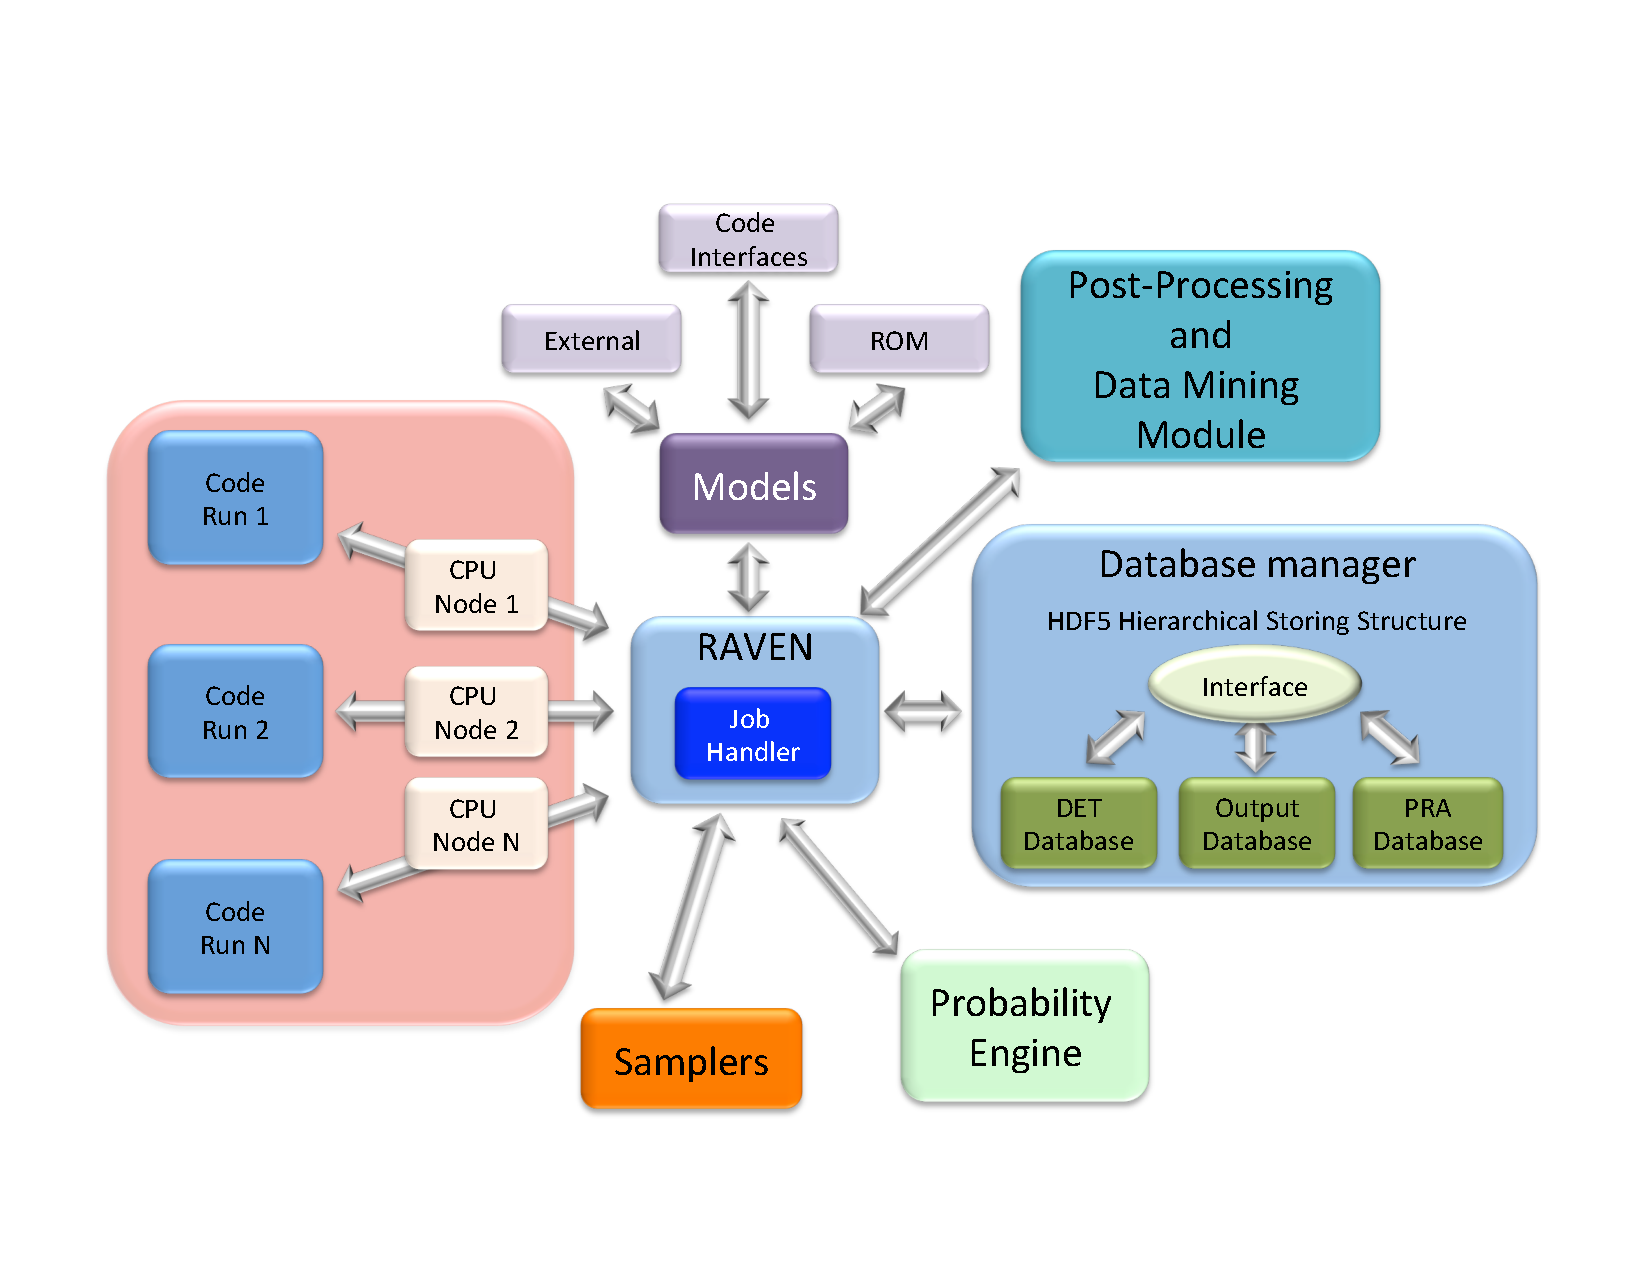
\includegraphics[scale=0.5]{raven.pdf}
    \caption{RAVEN}
    \label{fig:raven}
\end{figure}


\section*{References}

\bibliography{main}

\end{document}